% =============================================================================
%  Rapport — « Le stress se lit-il dans notre mode de vie ? »
%  Introduction to Data Processing — MAM3, Université Côte d'Azur, 2025-2026
%  Équipe : Hafssa, Thibaud, Nathan
%
%  Compilation : pdflatex (Overleaf par défaut). Pour un rendu typographique
%  optimal, XeLaTeX/LuaLaTeX fonctionnent aussi (garde iftex ci-dessous).
%      pdflatex report.tex   (×2 pour le sommaire/les références)
% =============================================================================
\documentclass[11pt,a4paper]{article}

\usepackage{iftex}
\ifpdftex
  \usepackage[utf8]{inputenc}
  \usepackage[T1]{fontenc}
\fi
\usepackage[french]{babel}
\usepackage[a4paper,margin=2.5cm]{geometry}
\usepackage{graphicx}
\usepackage{booktabs}
\usepackage{amsmath,amssymb}
\usepackage{xcolor}
\usepackage{pifont}      % \ding pour les verdicts ✓ / ✗
\usepackage{caption}
\usepackage{enumitem}
\usepackage[hidelinks]{hyperref}

\graphicspath{{figures/}}

% Couleurs cohérentes avec les figures : rouge = ↑ stress, bleu = ↓ stress
\definecolor{stressup}{HTML}{D1495B}
\definecolor{stressdown}{HTML}{3A6EA5}
\newcommand{\hot}[1]{\textcolor{stressup}{#1}}
\newcommand{\cool}[1]{\textcolor{stressdown}{#1}}
\newcommand{\cmark}{\textcolor{stressdown}{\ding{51}}}
\newcommand{\xmark}{\textcolor{stressup}{\ding{55}}}

\title{\textbf{Le stress se lit-il dans notre mode de vie ?}\\[2pt]
  \large Rapport --- \textit{Introduction to Data Processing} (MAM3, 2025-2026)}
\author{Hafssa \quad\textbullet\quad Thibaud \quad\textbullet\quad Nathan}
\date{Université Côte d'Azur --- Polytech Nice Sophia}

\begin{document}
\maketitle

\noindent\textbf{Dépôt Git :} \url{https://github.com/barbiernathan2005/PROJET-DATA-SCIENCE}\\
\textbf{Dataset :} \textit{Lifestyle \& Wellbeing Data} --- Kaggle (\texttt{ydalat}),
enquête Authentic-Happiness.

\medskip
\hrule
\medskip

% =============================================================================
\section{Business goal}
% =============================================================================

\noindent\textbf{Quel est notre dataset ? Pourquoi est-il utile ?}

\medskip
Notre projet répond à une question simple et universelle : \textbf{quels facteurs de
notre mode de vie sont liés à notre niveau de stress quotidien ?} Comprendre cela a
une valeur concrète pour les applications de bien-être, les programmes de prévention
santé et la qualité de vie au travail : si l'on identifie des leviers actionnables
(sommeil, congés, méditation\dots), on peut formuler des recommandations utiles.

Notre parcours a commencé par un \textbf{échec instructif}. Notre premier dataset
(\texttt{Global\_Mental\_Health\_Dataset\_2025.csv}, \textbf{2\,500 lignes}), sur la
« santé mentale », semblait idéal pour notre toute première problématique --- \textit{peut-on
prédire le stress à partir du sommeil ?} Mais à l'analyse, \textbf{aucune variable
n'était corrélée à une autre} : la corrélation maximale (hors diagonale) entre toutes
les variables numériques ne valait que $|r| \approx 0{,}04$, et le couple
sommeil\,$\leftrightarrow$\,stress tombait à $-0{,}02$ (Figure~\ref{fig:synth}). En
enquêtant, nous avons compris que ces données étaient \textbf{générées artificiellement},
pas mesurées : elles ne pouvaient rien nous apprendre. Nous avons aussi constaté que
tout le thème « stress / burnout » sur Kaggle est saturé de jeux de données
synthétiques. Première leçon, devenue notre fil rouge : \textit{vérifier la provenance
et la réalité des données avant toute analyse.}

\begin{figure}[h]
  \centering
  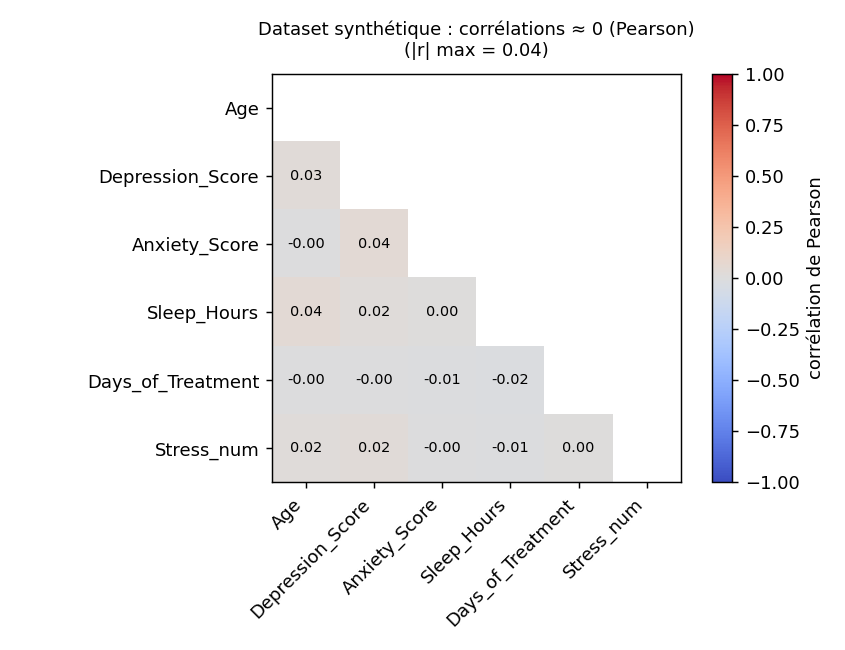
\includegraphics[width=0.62\linewidth]{00_probleme1_synthetique.png}
  \caption{Le dataset abandonné (synthétique). La matrice de corrélation est
    entièrement « éteinte » (toutes les cases $\approx 0$) : c'est la \textbf{signature
    de données fabriquées} --- aucune relation exploitable, donc aucune histoire à
    raconter, exactement l'inverse des données réelles (Figure~\ref{fig:corr}).}
  \label{fig:synth}
\end{figure}

Nous avons alors choisi un jeu de données \textbf{réel} : l'enquête \textit{Lifestyle
\& Wellbeing} d'Authentic-Happiness, soit \textbf{15\,971 réponses authentiques}
collectées dans le monde (2015-2020). Chaque répondant a renseigné ses habitudes de
vie et son niveau de stress quotidien. Contrairement au premier dataset, ces données
présentent de vraies relations exploitables --- et les imperfections typiques du réel
(une valeur erronée à corriger), gage d'authenticité.

% =============================================================================
\section{Team management}
% =============================================================================

\noindent\textbf{Comment travaillons-nous ? Quel est notre planning ?}

\medskip
Nous sommes une équipe de \textbf{3 personnes}, coordonnée via un \textbf{dépôt Git}
partagé.

\medskip
\noindent\textbf{Répartition des rôles :}
\begin{itemize}[nosep,leftmargin=1.4em]
  \item \textbf{Hafssa --- Données \& nettoyage :} chargement, sanity checks, encodage
    des catégories, gestion des valeurs manquantes.
  \item \textbf{Nathan --- Visualisation \& features maison :} figures, conception et
    justification des indices, vérification de leur pertinence.
  \item \textbf{Thibaud --- Modélisation \& storytelling :} régression, validation
    croisée, interprétation, rédaction du récit et des slides.
\end{itemize}

\medskip
\noindent\textbf{Planning (calendrier du cours) :}
\begin{center}
\begin{tabular}{@{}ll@{}}
  \toprule
  \textbf{Jour} & \textbf{Tâche} \\
  \midrule
  Lun.\ 01/06 & Définition du problème, choix et chargement des données \\
  Mar.\ 02/06 & Nettoyage, visualisation, première trame de storytelling \\
  Mer.\ 03/06 & Features maison, régression linéaire, itérations \\
  Jeu.\ 04/06 & Pipeline final, préparation de l'oral, dépôt des slides \\
  Ven.\ 05/06 & Soutenance orale + finalisation du rapport \\
  \bottomrule
\end{tabular}
\end{center}

\medskip
Les décisions importantes (choix du dataset, des features, message clé) ont été prises
\textbf{collectivement}.

% =============================================================================
\section{Data visualisation}
% =============================================================================

\noindent\textbf{Description.} Le dataset contient \textbf{15\,971 lignes} et
\textbf{23 variables}. La cible est \texttt{DAILY\_STRESS}, un score de stress
quotidien de \textbf{0 (aucun) à 5 (très stressé)}, traité comme continu. Les
explicatives sont de deux types :
\begin{itemize}[nosep,leftmargin=1.4em]
  \item \textbf{$\sim$20 variables numériques} de mode de vie : \texttt{SLEEP\_HOURS},
    \texttt{DAILY\_STEPS}, \texttt{SOCIAL\_NETWORK}, \texttt{CORE\_CIRCLE},
    \texttt{SUPPORTING\_OTHERS}, \texttt{WEEKLY\_MEDITATION}, \texttt{FLOW},
    \texttt{TIME\_FOR\_PASSION}, \texttt{LOST\_VACATION}, \texttt{DAILY\_SHOUTING},
    \texttt{SUFFICIENT\_INCOME}, \texttt{PERSONAL\_AWARDS}, etc. ;
  \item \textbf{2 variables catégorielles} : \texttt{AGE} (tranches) et \texttt{GENDER}.
\end{itemize}

\noindent\textbf{Nettoyage (data wrangling).} La cible contenait une valeur non
numérique (\texttt{'1/1/00'}), forcée en \texttt{NaN} puis retirée (15\,971 lignes
conservées). \texttt{AGE} et \texttt{GENDER} ont été encodées en \textbf{one-hot}
(éviter un faux ordre), et toutes les variables \textbf{standardisées} (moyenne 0,
écart-type 1) pour comparer l'importance des coefficients.

\begin{figure}[h]
  \centering
  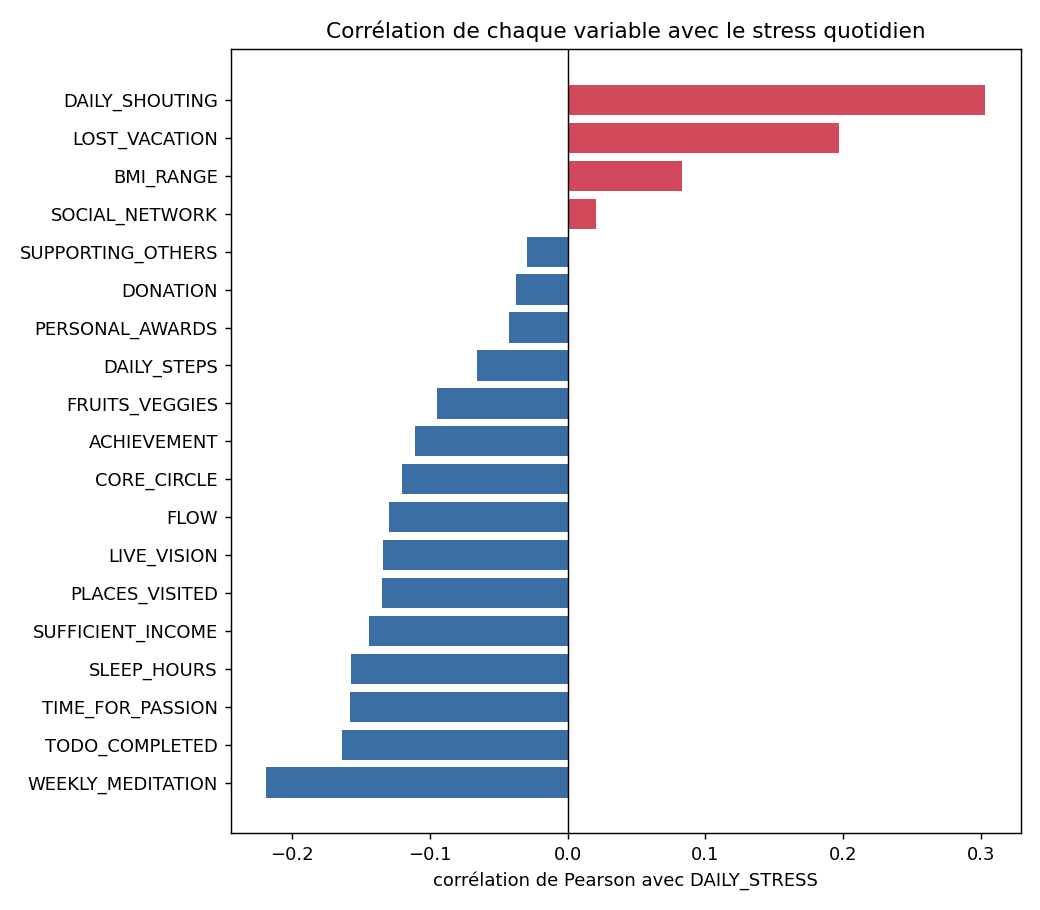
\includegraphics[width=0.70\linewidth]{01_correlations.png}
  \caption{Corrélation de chaque variable avec le stress. Barres horizontales triées
    (\hot{rouge} = corrélation positive, \cool{bleu} = négative), axe partant de zéro,
    palette à deux couleurs. \textit{Lecture :} aucune variable ne domine --- les
    corrélations sont \textbf{modérées} ---, ce qui motive notre travail de combinaison
    (section~\ref{sec:features}). Du côté « stress » ressortent \texttt{DAILY\_SHOUTING}
    et \texttt{LOST\_VACATION} ; du côté « apaisement », \texttt{WEEKLY\_MEDITATION},
    \texttt{SLEEP\_HOURS} et \texttt{SUFFICIENT\_INCOME}.}
  \label{fig:corr}
\end{figure}

\begin{figure}[h]
  \centering
  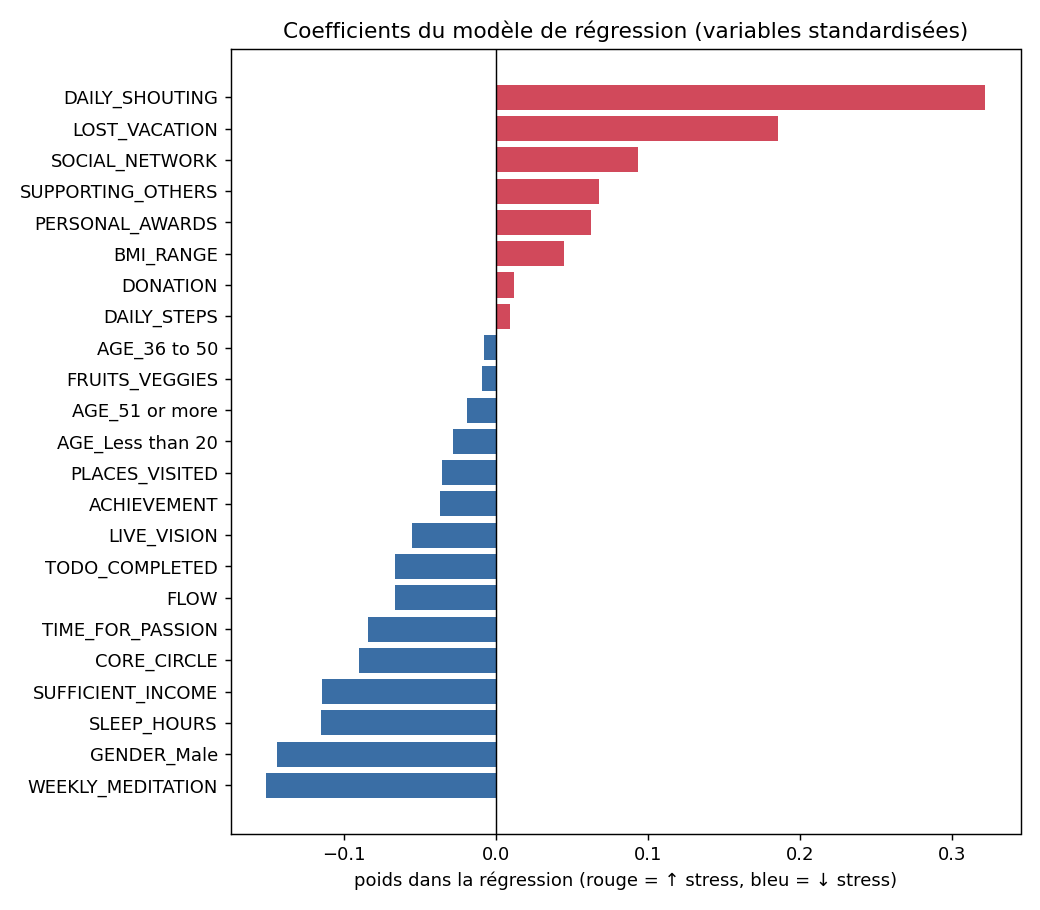
\includegraphics[width=0.70\linewidth]{02_coefficients_base.png}
  \caption{Coefficients du modèle (variables standardisées) : poids et signe de chaque
    variable dans la régression. \textit{Lecture :} répond visuellement à la question
    business --- qui fait \hot{monter} ou \cool{baisser} le stress.}
  \label{fig:coefbase}
\end{figure}

\noindent\textit{(Choix : des diagrammes en barres triés plutôt qu'un camembert ou un
nuage surchargé, car l'œil compare mieux des longueurs que des angles --- principe vu
en cours.)}

% =============================================================================
\section{Handcrafted features}\label{sec:features}
% =============================================================================

Le constat de la section précédente --- aucune variable seule n'est fortement corrélée
au stress --- nous a conduits à \textbf{construire 4 nouvelles variables} combinant les
variables brutes selon des hypothèses de bon sens :

\begin{enumerate}[leftmargin=1.6em]
  \item \texttt{SOCIAL\_SUPPORT} $=$ \texttt{CORE\_CIRCLE} $+$ \texttt{SOCIAL\_NETWORK}
    $+$ \texttt{SUPPORTING\_OTHERS}. \textit{Hypothèse :} le soutien social amortit le
    stress (Cohen \& Wills, 1985).
  \item \texttt{HEALTHY\_HABITS} $=$ \texttt{SLEEP\_HOURS} $+$ \texttt{DAILY\_STEPS}
    $+$ \texttt{WEEKLY\_MEDITATION} $+$ \texttt{FRUITS\_VEGGIES}. \textit{Hypothèse :}
    une même hygiène de vie, dont les comportements se cumulent.
  \item \texttt{OVERWORK} $=$ \texttt{LOST\_VACATION} $+$ \texttt{DAILY\_SHOUTING}
    $-$ \texttt{TIME\_FOR\_PASSION}. \textit{Hypothèse :} proxy de surmenage (beaucoup
    de congés non pris et d'irritabilité, peu de temps pour soi).
  \item \texttt{SLEEP\_x\_FLOW} $=$ \texttt{SLEEP\_HOURS} $\times$ \texttt{FLOW}.
    \textit{Hypothèse :} une \textbf{interaction} (produit, comme
    \texttt{Pclass}\,$\times$\,\texttt{Age} du cours) : bien dormir \textbf{et} être
    souvent absorbé a un effet protecteur \textbf{combiné}.
\end{enumerate}

\noindent\textbf{Vérification de la pertinence (corrélation avec le stress) :}
\begin{center}
\begin{tabular}{@{}lcl@{}}
  \toprule
  \textbf{Feature maison} & \textbf{Corrélation} & \textbf{Verdict} \\
  \midrule
  \texttt{OVERWORK}       & $\hot{+0{,}349}$  & \cmark\ le \textbf{signal le plus fort de toute l'étude} \\
  \texttt{HEALTHY\_HABITS}& $\cool{-0{,}218}$& \cmark\ pertinent (habitudes saines $\to$ moins de stress) \\
  \texttt{SLEEP\_x\_FLOW} & $\cool{-0{,}157}$& \cmark\ pertinent (l'interaction fonctionne) \\
  \texttt{SOCIAL\_SUPPORT}& $\cool{-0{,}055}$& \xmark\ quasi nul --- \textbf{échec instructif} \\
  \bottomrule
\end{tabular}
\end{center}

\medskip
\textbf{Trois indices sur quatre sont très pertinents} --- \texttt{OVERWORK} dépasse
même toutes les variables brutes. Mais \texttt{SOCIAL\_SUPPORT} \textbf{échoue}, et ce
résultat est le plus riche d'enseignement. En inspectant ses composantes
(Figure~\ref{fig:coefbase}), on voit qu'elles se \textbf{contredisent} : un grand
réseau social (\texttt{SOCIAL\_NETWORK}, coef.\ $\hot{+0{,}09}$) et le fait d'aider
beaucoup les autres (\texttt{SUPPORTING\_OTHERS}, $\hot{+0{,}07}$) vont de pair avec
\textbf{plus} de stress --- sans doute parce que les personnes très sollicitées
socialement sont aussi plus occupées/stressées. En les additionnant avec l'entourage
proche, les effets s'annulent. \textbf{Leçon :} une feature combinée n'est utile que si
ses composantes pointent dans le même sens --- la vérification de pertinence sert
précisément à le détecter.

\begin{figure}[h]
  \centering
  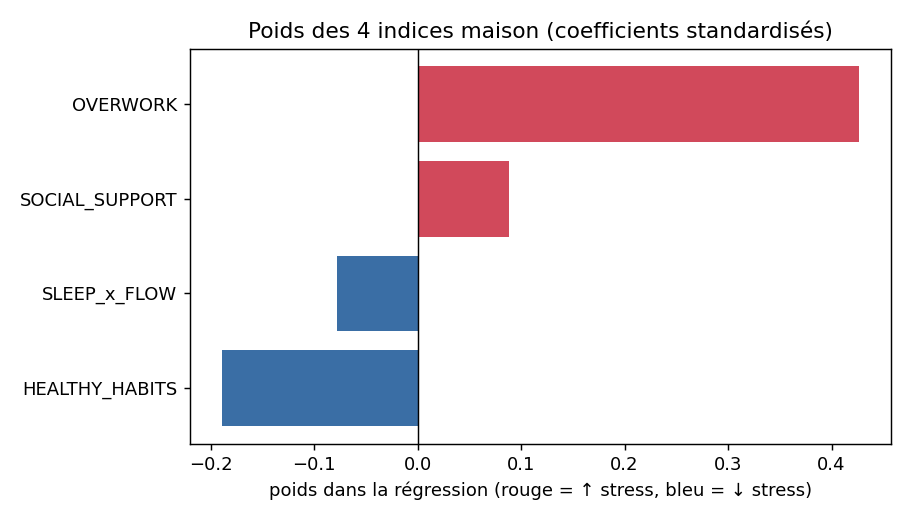
\includegraphics[width=0.62\linewidth]{03_coefficients_indices.png}
  \caption{Poids des 4 indices maison (coefficients standardisés).}
  \label{fig:coefind}
\end{figure}

% =============================================================================
\section{Linear / logistic / softmax regression}
% =============================================================================

\noindent\textbf{Choix : la régression linéaire.} La cible (\texttt{DAILY\_STRESS},
0-5) est numérique et ordonnée ; nous la traitons comme \textbf{continue}. Surtout,
notre objectif est l'\textbf{explication} (comprendre les leviers) plus que la
prédiction parfaite : les coefficients d'une régression linéaire s'\textbf{interprètent
directement}.

\medskip
\noindent\textbf{Méthode.} $\text{stress} \approx \beta_0 + \beta_1 x_1 + \dots +
\beta_k x_k$, coefficients estimés par \textbf{moindres carrés} (solution des équations
normales $\hat{\beta} = (A^\top A)^{-1} A^\top y$, vue en cours).

\medskip
\noindent\textbf{Protocole (validation).} Découpage \textbf{train/test 80-20} ;
\textbf{standardisation} apprise sur le train ; \textbf{validation croisée 5-fold} pour
une estimation robuste.

\medskip
\noindent\textbf{Résultats.}
\begin{itemize}[nosep,leftmargin=1.4em]
  \item $R^2$ (modèle à 23 variables, test) $=$ \textbf{0,187}
  \item $R^2$ (modèle à 4 indices maison, test) $=$ \textbf{0,125} ; en
    \textbf{5-fold $=$ 0,143 $\pm$ 0,013}
  \item \hot{\textbf{Font monter}} le stress : \texttt{DAILY\_SHOUTING}
    ($\hot{+0{,}32}$), \texttt{LOST\_VACATION} ($\hot{+0{,}18}$), \texttt{SOCIAL\_NETWORK}
    ($+0{,}09$), \texttt{PERSONAL\_AWARDS} ($+0{,}06$).
  \item \cool{\textbf{Font baisser}} le stress : \texttt{WEEKLY\_MEDITATION}
    ($\cool{-0{,}15}$), \texttt{GENDER\_Male} ($-0{,}15$), \texttt{SLEEP\_HOURS}
    ($-0{,}13$), \texttt{SUFFICIENT\_INCOME} ($-0{,}12$), \texttt{TIME\_FOR\_PASSION}
    ($-0{,}09$).
\end{itemize}

\medskip
\noindent\textbf{Interprétation.} Le mode de vie explique environ \textbf{15 à 19\,\%
de la variance} du stress. Le facteur le plus fort, \texttt{DAILY\_SHOUTING}, est à
manier avec prudence : crier/bouder est en partie un \textbf{symptôme} du stress, pas
seulement une cause (relation quasi-circulaire). Le facteur aggravant le plus
\textbf{actionnable} est \texttt{LOST\_VACATION} (ne pas prendre ses congés). À
l'inverse, \textbf{méditer, dormir, avoir un revenu suffisant et du temps pour ses
passions} sont associés à moins de stress. On note aussi que les hommes déclarent un
stress un peu plus faible (\texttt{GENDER\_Male} $-0{,}15$).

\medskip
\noindent\textbf{Fiabilité.} Le $R^2$ est \textbf{modéré}, ce qui est \textbf{attendu
et honnête} : le stress est multifactoriel et auto-déclaré. La \textbf{stabilité} du
5-fold (écart-type 0,013) indique un modèle \textbf{non sur-appris}. Le modèle à 4
indices est un peu moins performant que le modèle complet (0,13 vs 0,19) : c'est le
\textbf{compromis} interprétabilité / performance --- on conserve environ \textbf{deux
tiers} du pouvoir explicatif avec \textbf{5 fois moins} de variables. Nous avons enfin
\textbf{écarté} \texttt{WORK\_LIFE\_BALANCE\_SCORE} (somme des autres colonnes) pour
éviter un $R^2$ artificiellement parfait (fuite d'information).

% =============================================================================
\section{Conclusion}
% =============================================================================

\noindent\textbf{Bénéfices.} L'analyse montre qu'une part du stress quotidien
\textbf{s'explique par le mode de vie} et désigne des \textbf{leviers concrets} :
prendre ses congés, méditer, dormir, se garder du temps pour ses passions. Notre
feature \texttt{OVERWORK} (surmenage) s'est révélée le \textbf{meilleur prédicteur} de
toute l'étude (corrélation $+0{,}35$).

\medskip
\noindent\textbf{L'enseignement le plus précieux} est venu d'un \textbf{échec} : la
feature \texttt{SOCIAL\_SUPPORT}, pourtant fondée sur la littérature, n'explique rien
ici --- parce que ses composantes se contredisent dans ces données. Cela rappelle qu'une
hypothèse doit toujours être \textbf{vérifiée empiriquement}.

\medskip
\noindent\textbf{Limites :} données \textbf{auto-déclarées} (biais de perception),
cible grossière 0-5, et surtout \textbf{corrélation $\neq$ causalité}.

\medskip
\noindent\textbf{Améliorations :} (i) une \textbf{régression ordinale/logistique}
adaptée à l'échelle 0-5 ; (ii) revoir \texttt{SOCIAL\_SUPPORT} en séparant entourage
proche et réseau étendu ; (iii) \textbf{segmenter par âge/genre} ; (iv) des données
longitudinales pour approcher la causalité.

\medskip
\noindent\textbf{La vraie leçon du projet :} des données \textit{réelles} racontent une
histoire --- y compris quand elles contredisent nos hypothèses ; des données
\textit{fabriquées}, non. Savoir faire la différence est la première compétence du data
scientist.

% =============================================================================
\section{List of references}
% =============================================================================

\begin{enumerate}[leftmargin=1.6em]
  \item \textbf{Dataset.} \textit{Lifestyle and Wellbeing Data}, Kaggle
    (\textit{ydalat}). \url{https://www.kaggle.com/ydalat/lifestyle-and-wellbeing-data}
    --- enquête « How's Life? The Work-Life Balance survey », www.authentic-happiness.com.
  \item \textbf{Cours.} L.\ Fillatre, \textit{Introduction to Data Processing},
    Université Côte d'Azur, Polytech Nice Sophia, 2025-2026 (Lectures 1 à 4).
  \item \textbf{scikit-learn.} Pedregosa et al., \textit{Scikit-learn: Machine Learning
    in Python}, JMLR 12, 2011. \url{https://scikit-learn.org/stable/modules/linear_model.html}
  \item \textbf{pandas.} McKinney, \textit{Data Structures for Statistical Computing in
    Python}, 2010.
  \item \textbf{Visualisation.} C.\ O.\ Wilke, \textit{Fundamentals of Data
    Visualization}, O'Reilly, 2019. \url{https://clauswilke.com/dataviz/}
  \item \textbf{Soutien social \& stress.} S.\ Cohen \& T.\ A.\ Wills, « Stress, social
    support, and the buffering hypothesis », \textit{Psychological Bulletin}, 98(2),
    1985, p.\ 310-357.
\end{enumerate}

\end{document}
